%% ----------------------------------------------------------------
%% Thesis.tex -- MAIN FILE (the one that you compile with LaTeX)
%% ----------------------------------------------------------------

% Set up the document
\documentclass[12pt,a4paper,oneside]{csedu}  % Use the "Thesis" style, based on the ECS Thesis style by Steve Gunn
\graphicspath{{Figures/}}  % Location of the graphics files (set up for graphics to be in PDF format)

% Include any extra LaTeX packages required
\usepackage{graphicx}
\usepackage[square, numbers, comma, sort&compress]{natbib}  % Use the "Natbib" style for the references in the Bibliography
\usepackage{verbatim}  % Needed for the "comment" environment to make LaTeX comments
\usepackage{vector}  % Allows "\bvec{}" and "\buvec{}" for "blackboard" style bold vectors in maths
\hypersetup{urlcolor=black, colorlinks=true}  % Colours hyperlinks in blue, but this can be distracting if there are many links.
\usepackage{algorithm} % for writing pseducode
\usepackage{algorithm,algpseudocode}
\usepackage{amsthm}
\usepackage{array}
\usepackage{tabularx}

%% ----------------------------------------------------------------
\begin{document}
\frontmatter      % Begin Roman style (i, ii, iii, iv...) page numbering

% Set up the Title Page
\title{Sliding Window Based Infrequent Weighted Itemset Mining}
\authors  %{\texorpdfstring
         %{\href{your web site or email address}{Name}}
{Abdullah Al - Matin  \\Exam Roll: Curzon Hall-- 1085\\Registration No: Ha - 895}
%{Your name should not appear on the external copies, write name between braces on the left}


%      {Author Name}
%   }
%\addresses  {\groupname\\\deptname\\\univname\\\FACULTY}  % Do not change this here, instead these must be set in the "Thesis.cls" file, please look through it instead, add roll, session and registration number ehich starts at line 204.
%\date       {\today}
%\subject    {}
%\keywords   {}

\maketitle

%% ----------------------------------------------------------------

\setstretch{1.5}  % It is better to have smaller font and larger line spacing than the other way round

% Define the page headers using the FancyHdr package and set up for one-sided printing
\fancyhead{}  % Clears all page headers and footers
\rhead{\thepage}  % Sets the right side header to show the page number
\lhead{}  % Clears the left side page header

\pagestyle{fancy}  % Finally, use the "fancy" page style to implement the FancyHdr headers

%% ----------------------------------------------------------------
% Declaration Page required for the Thesis, your institution may give you a different text to place here
\Declaration{

\addtocontents{toc}{\vspace{1em}}  % Add a gap in the Contents, for aesthetics

I, hereby, declare that the work presented in this project is the
outcome of the investigation performed by me under the supervision
of Dr. Chowdhury Farhan Ahmed, Associate Professor, Department of Computer
Science and engineering, University of Dhaka. I also declare that
no part of this project has been or is being submitted elsewhere
for the award of any degree or diploma.

\bigskip
\bigskip
\bigskip


%\begin{tabular}{lp{1in}r}
%\\ & \\ & \\


\begin{tabular}{c c c c}

  % after \\: \hline or \cline{col1-col2} \cline{col3-col4} ...
  Countersigned &\hspace{1.8in} & & Signature \\

   & & &  \\
  \ldots\ldots\ldots\ldots \ldots\ldots\ldots\ldots   & & & \ldots\ldots\ldots\ldots \ldots\ldots\ldots\ldots   \\
  (Dr. Chowdhury Farhan Ahmed) & & & (Abdullah Al - Matin) \\
  {\bf Supervisor} & & &  \\

 

\end{tabular}
}

\clearpage  % Declaration ended, now start a new page



% The Abstract Page
\addtotoc{Abstract}  % Add the "Abstract" page entry to the Contents
\abstract{
Now a days, frequent itemset mining is a popular approach. For finding frequent itemset, several approaches is already established. Infrequent items can be also very important for finding unexpected behavior like fraud detection, cost function minimization, equal task distribution for data center resource management etc. Weight may play a very important role in this scenario. In general approach, weighted itemset is treated all alike. But we have proposed an algorithm for mining infrequent weighted itemset by treating them differently based on their weight. Experimental results and graphs are added for the support of our proposed algorithm’s efficiency and effectiveness.
\addtocontents{toc}{\vspace{1em}}  % Add a gap in the Contents, for aesthetics

 }

\clearpage  % Abstract ended, start a new page
%% ----------------------------------------------------------------

\setstretch{1.3}  % Reset the line-spacing to 1.3 for body text (if it has changed)

% The Acknowledgements page, for thanking everyone
\acknowledgements{
\addtocontents{toc}{\vspace{.5em}}  % Add a gap in the Contents, for aesthetics
%
%
First of all, I am thankful and expressing my gratefulness to Almighty Allah who offers me His divine blessings, patient, mental and psychical strength to complete this project work.
%
I am deeply indebted to my project supervisor Dr. Chowdhury Farhan Ahmed, Associate Professor, Department of Computer Science and
Engineering, University of Dhaka. His scholarly guidance,
important suggestions, endless patience, constant supervision,
valuable criticism, and enormous amount of work for going through
my drafts and correcting them, and generating courage from the
beginning to the end of the research work has made the completion
of the project possible.\\
%
I would like to express my deep gratitude to Md. Samiullah
and Muhammed Tawfiqul Islam, lecturer, Dept of CSE DU for his
support and help for my work. The discussions with him on various
topics related my works have helped me to enrich my knowledge
and conception regarding this work.\\
%
Last but not the least; I am highly grateful to my parents and
family members for their support and constant encouragement, which
have always been a source of great inspiration for me.
}
\clearpage  % End of the Acknowledgements
%% ----------------------------------------------------------------

\pagestyle{fancy}  %The page style headers have been "empty" all this time, now use the "fancy" headers as defined before to bring them back


%% ----------------------------------------------------------------
\lhead{\emph{Contents}}  % Set the left side page header to "Contents"
\tableofcontents  % Write out the Table of Contents

%% ----------------------------------------------------------------
\lhead{\emph{List of Figures}}  % Set the left side page header to "List if Figures"
\listoffigures  % Write out the List of Figures

%% ----------------------------------------------------------------
\lhead{\emph{List of Tables}}  % Set the left side page header to "List of Tables"
\listoftables  % Write out the List of Tables

%% ----------------------------------------------------------------
\setstretch{1.5}  % Set the line spacing to 1.5, this makes the following tables easier to read
\clearpage  % Start a new page
%\lhead{\emph{Abbreviations}}  % Set the left side page header to "Abbreviations"
%\listofsymbols{ll}  % Include a list of Abbreviations (a table of two columns)
%{
% \textbf{Acronym} & \textbf{W}hat (it) \textbf{S}tands \textbf{F}or \\
%\textbf{LAH} & \textbf{L}ist \textbf{A}bbreviations \textbf{H}ere \\

%\textbf{} & \textbf{} \textbf{} \textbf{} \\
%}

%% ----------------------------------------------------------------
\clearpage  % Start a new page


\setstretch{1.5}  % Return the line spacing back to 1.3

\pagestyle{empty}  % Page style needs to be empty for this page
%\dedicatory{For/Dedicated to/To my\ldots}

\addtocontents{toc}{\vspace{2em}}  % Add a gap in the Contents, for aesthetics


%% ----------------------------------------------------------------
\mainmatter   % Begin normal, numeric (1,2,3...) page numbering
\pagestyle{fancy}  % Return the page headers back to the "fancy" style

% Include the chapters of the thesis, as separate files
% Just uncomment the lines as you write the chapters

% Chapter 1
\chapter{Introduction}
% Write in your own chapter title\label{Chapter 1}
\lhead{Chapter 1. \emph{Introduction}}
 % Write in your own chapter title to set the page header
%\section{Data mining}
 %
Data mining is the process for finding interesting and useful patterns from a dataset. The very first approach was finding frequent items i.e. the items that are used frequently. It plays an important role for finding knowledge discovery technique such as association rule mining, classification, clustering, time-series mining, graph mining, web mining etc. A lots of research and algorithm have been proposed for finding frequent patterns using Apriori based algorithms, FP tree based algorithms and others algorithms. In real life, frequent item set finding application is used in market basket analysis [], medical image processing [], biological data analysis [] etc. Traditionally, all items in a transaction are treated equally. Though all items interest/influence is not same, they should be treated differently. For solving this problem, the notion of weighted item set mining has been introduced []. The weight of an item is the value that signifies the local interest within each transaction. 
\par
Several approaches have been proposed for IWIM (Infrequent Weighted Itemset Mining). In those approaches, they consider all data from the very beginning of the database. Therefore these approaches cannot be applicable for a large-scale data set such as data streams [] where data set flows in the form of continuous stream. Data stream is a continuous, unbound and ordered sequence of items that comes in order of time. In this case, it is impossible to maintain all data from the dataset and cannot possible to process all data at a time.  
\par
Existing algorithm works on whole fixed dataset and generates infrequent item set. For data stream, it have handle data in an efficient manner. Older data will be lost and also new updated data have to process. So it should differentiate recently generated data from older information which may unimportant or obsolete in context of time.
\par
Consider as an example, the data set in Table~\ref{tab:Table} where there is a set of transactions from data stream. Here we have considered a small part of the data set for simplicity. It contains eight transactions. These transactions are identified by tids. Each transaction contains four distinct items with their weights. It’s not necessary to be exact four items. Weight is defined by the corresponding degree of interest in the transaction i.e. item {\it b} contains weight 43 in tid 2 but in tid 3 is 0. Item weight is the value of CPU usage readings at a specific time. For data stream this CPU usage reading is done at a fixed sampling rate. This CPU usage is important for data center resource management and application specific profiling. In tid4, weight of item {\it a} is 100. It means CPU a is working at high usage rate. While in tid 1, its weight is 0. It means temporarily {\it a} is idle. Knowledge extracting from this data set is important for domain expert or specific application expert to allocate system task break down for all CPU at a specific time.  So that, the system output can be maximized.
%

\begin{table}
\begin{center}
\begin{tabular}{ |c|c| } 
\hline
Transaction IDs (tid) & CPU usage reading \\
\hline
1 & (a,0) (b,100) (c,57) (d,71)\\
2 & (a,0) (b,43) (c,29) (d,71)\\
3 & (a,43) (b,0) (c,43) (d,43)\\
4 & (a,100) (b,0) (c,43) (d,100)\\
5 & (a,86) (b,71) (c,57) (d,71)\\
6 & (a,57) (b,71) (c,0) (d,71)\\
7 & (a,91) (b,32) (c,11) (d,0)\\
8 & (a,17) (b,61) (c,0) (d,72)\\
\hline
\end{tabular}
\caption{Example of a transaction data stream with weight}
\label{tab:Table}
\end{center}
\end{table}





%\begin{figure}[ht]
%\centering
%\includegraphics {transactions.eps}
%\caption{Transaction}
%\label{fig:trans}
%\end{figure}
%


%
%

\iffalse
\section{Basic Concepts}
 %
The main approaches of data mining include:\\
\textbf{Frequent pattern, association and correlation mining:}
Frequent patterns are patterns that frequently occur in data. There are many kinds of frequent patterns, including itemsets, subsequences, and substructures. For example, if milk and bread are frequently bought items in a market, then $\{milk, bread\}$ is a frequent itemset. 
Association rule mining finds interesting relationships among a large set of data items. The association rules are considered interesting if they satisfy both a minimum support threshold and a minimum confidence threshold \cite{book}.
Correlation analysis is a measure which finds the underlying dependencies between itemsets of data.\\
%
\textbf{Classification:}
Classification is the problem of identifying to which of a set of categories a new data belongs. It is done on the basis of a training set of data whose class label is known.\\
%
\textbf{Cluster Analysis:}
Cluster analysis deals with data for which the class labels are not known. Here, data is clustered or grouped based on the principle of maximizing the intraclass similarity and minimizing the interclass similarity \cite{book}. \\
%
\textbf{Outlier Analysis:}
A data set may contain some data which behaves differently than the rest of the data. This type of data is known as outlier. Sometimes this outliers provides us with useful information about the dataset. Analysis of these outlier data is known as outlier analysis.  
%
\section{Infrequent Itemset Mining} \label{sec:graph_mining}
%
Frequent itemset mining is a very common approach for finding frequent items. In our approach, we are trying to find infrequent items. Those  are the infrequent items, whose value is below threshold. For a given max{\_}support value, items value is below the max{\_}support. Infrequent item is important for resource management, application profiling, and fraud detection. It can be used for finding any unexpected or abnormal behaviour of a system. 

%
%\begin{figure}[ht]
%\centering
%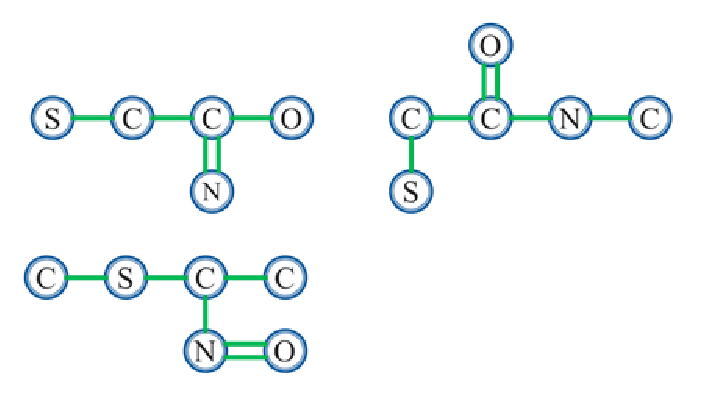
\includegraphics[scale = 0.8] {graph_data.eps}
%\caption{a set of chemical compounds represented using graph}
%\label{fig:graphdata}
%\end{figure} 
%
%
\fi


\section{Motivation}
%
Mining for infrequent itemset is recently gained attention of research community. Main focus for finding infrequent itemset whose frequency value is below \texttt{max\_support}. Not only frequency, weight can be also used for finding infrequent itemset mining. \\

\par
Let’s consider a scenario. A banking system where lots of transactions is done every day. As a bank officer, one may want to know if everything okay or not. In general cases, all transactions are okay but in fraud cases or unexpected cases, it may vary. It’s difficult for a bank officer to browse all data of the transactions to find any abnormal cases every day. It’s pretty hard for him. \\
\iffalse
%
\par \textbf{Motivating scenario:} \\
An application domain of graph classification related to the context of Bangladesh is drug discovery. Drug design and discovery is a growing field of interest in Bangladesh. The goal in drug discovery is to analyze this huge chemical space and identify molecules that show a certain desired activity. However, given the magnitude of the chemical space, an exhaustive exploration is not feasible \cite{drug}. Graph classification can be effectively used in this domain for molecular classification. \\
%
%\par The main goal of a graph classification approach is to classify graphs accurately and efficiently. But if we see some of the existing works we will find that, \\
%

\begin{itemize}
\item GAIA \cite{gaia} is a graph classification approach that makes use of evolutionary computation for feature selection purpose. But, it selects features by assigning  a score to a subgraph by only considering its own occurrence in the positive/negative graphs, it does not consider any other parameters. For this reason, its performance in terms of accuracy is not sufficient.
%
\item D\&D \cite{dnd} is one of the latest works in the field of graph classification. It provides a diversified discriminative score based on edge cover probability to select features. However, its performance is still not at satisfactory level. There is scope of improvement in terms of accuracy and runtime.
\end{itemize}
%
The above mentioned lackings of the existing works motivate us to develop a better graph classification approach.
%
\fi
\section{Objective}
%
We have studied that the existing approaches are limited to some context. As a solution, we have to develop an algorithm that can overcome the limitations. The objectives of our work are listed below:
%
\begin{itemize}
\item To carry out an extensive literature view regarding the infrequent itemset mining approach.
\item Propose a new efficient algorithm for finding infrequent items. 
\item Propose an algorithm that can perform in broader area.
\end{itemize}
%
\section{Thesis Contribution}
%
The contributions our research work are listed below:
%
\begin{itemize}
%
\item We have used sliding window based approach. This reduces the processing time \& memory space for pressing.
%
\item We can get the actual contribution of an item in the dataset. Previous approach uses equivalence weighting function for data items.
% 
\item It’s easier to discard frequent items from the candidate infrequent pattern list.
\item Extra cost for checking infrequent patterns validation i.e. is the item actually infrequent or not.
%
\end{itemize}
%
\section{Thesis Outline}
The five chapters labeled as Introduction, Related Work, Proposed Approach, Performance Evaluation and Conclusion form the shape of the book.
Every chapter comprises of the following topics: \\
%
Chapter 1 contains some introductory concepts such as data mining and various data mining approaches, infrequent itemset mining and also the motivation and contribution of this work.\\
%
Chapter 2 describes various terms related to previous work in the field of infrequent itemset mining and also the limitations of the existing approaches. \\
%
Chapter 3 describes the proposed score and algorithm. It also contains the details of our work and application of the proposed algorithm. \\
%
Chapter 4 contains the implementation results and performance evaluation results of the proposed algorithm. \\
%
Chapter 5 draws the conclusion of the thesis by summarizing the
findings in the thesis and describing scope of possible extensions to this work. \\
%
The last part of the book is Bibliography which places all the reference cited in the work. The appendix works as additional information that helps the reader if necessary.
%
 % Introduction

% Chapter 3
\chapter{Previous Works} % Write in your own chapter title
\label{Chapter 2}
\lhead{Chapter 2. \emph{Previous Works}} 
In this chapter, we discuss some basic terminologies and background knowledge in infrequent itemset mining, sliding window based approach and Share-frequent approach. 
We also discuss some recent works in the field of infrequent itemset mining. Here, we highlight their working procedure and analyze the algorithms.
\section{Related Works}
Frequent itemset mining is commonly used and established process for finding frequent items \cite{agrawal1993mining}. In general approaches, all items in a dataset is treated equally. But when an item is having weight, 
it can�t be treated equally with other items. If we do so, we will lose more information from the dataset. For differentiating the itemsets, \cite{wang2000efficient} authors focus on finding more informative association 
rules. This rule is named �Weighted association rules� (WAR). In this approach, weight denotes the significance of an item.  Based on weight, items are processed for mining. Mining process is also 
done by keeping weight in mind. Weight can be pre-assigned or not. Several approaches have been already established \cite{tao2003weighted}, \cite{wang2000efficient}.  Based on weight, infrequent itemset mining has also gained interest. Those itemsets 
are infrequent that frequency is less than min\_support. Their frequency is also quite little. In \cite{cagliero2014infrequent}, minimal infrequent itemsets are mined. In this approach, they have taken a weighted dataset. 
Gives every item an equivalence weight for simplicity. Then they have created a weighted tree. This weighted is sent for mining. In mining process, they have applied FP-Growth like algorithm for 
finding infrequent itemsets. In their approach, tree construction is conducting more time. It also creates the tree more branches. Mining process shows infrequent items but they cannot provide the 
actual contribution of an item in the dataset. This approach works on a fixed dataset and cannot be applied for stream data.\\

Sliding window is an approach for processing stream data. In stream data, data is a continuous channel and arrives within a fixed time range. So, it requires to process those data within a very small 
span of time. In \cite{ahmed2009efficient}, an efficient approach is proposed for finding frequent items using sliding window mechanism. It introduces the idea of window size and batch size. Each batch contains a numbers of 
transactions. Window size is the number of batches. Window slides to next window new batches come. As previous data are no longer present, so it deletes the previous data and its related weight from table.
It constructs the tree for a window and perform mining process. When a window is completed, it slides to next.\\ 

Let, {\it I} = \{{\it $i_1$, $i_2$,. . . . . ,$i_m$}\} be a  set of items and T be a transaction database Transactional dataset {\it D} =\{{\it $T_1$, $T_2$, $T_3$,. . . . . ,$T_n$}\} where each transaction Ti D is a subset of I. 
The support of an item is the number of transaction containing the item in the transactional database. To find frequent items, items should satisfy the minimum support in the transaction database. The downward closure property (Agarwal et al., 1993; 
Agarwal and Srikant, 1994) is used prune the infrequent items. This property ensures that if an item is infrequent then its supper set must be infrequent. In our approach, we are targeting these 
infrequent items. Apriori (Agarwal et al., 1993; Agarwal and Srikant, 1994) algorithm is widely used for mining frequent items and very useful in association rule mining. But candidate generation 
and test, several database scan are the side effect of appriori algorithm.  FP-growth (Han et al., 2004) algorithm solves the problem of candidate generation and test. It requires only two database scan.\\

To discover useful knowledge about numerical attributes associated with items in a transaction, Carter et al., 1997 first introduced the share-confidence model. SIP, CAC and 
IAN (Barber and Hamilton, 2000, 2001, 2003) have been proposed but they may not discover all shared-frequent patterns. Several approaches have been also proposed to resolve the discovery of all 
frequent items and that also maintain the downward closure property. In [], an effective approach is described,\\

The existing weighted infrequent pattern mining methods consider all transactions of a database from the very beginning and requires extra database scan. Hence, they are not appropriate for data 
stream. They can�t find recent interesting information from the dataset. Therefore, we have proposed sliding window based novel algorithm for single-pass weighted infrequent pattern mining to extract 
the recent change of knowledge in a data stream adaptively. We have also applied the ShrFP-Tree approach to find the actual contribution of a pattern.\\ % Previous Work

% Chapter 3

\chapter{Proposed Approach} % Write in your own chapter title
\label{Chapter 3}
\lhead{Chapter 3. \emph{Proposed Approach}} % Write in your own chapter title to set the page header
In this chapter we present our proposed approach for finding infrequent itemset mining over data stream. We discuss about the definition, process and algorithms of our proposed approach. 
%\section{Introduction}
%
%\section{Terminologies}
%
%\section{Problem Definition and Solution Methodology}
%
\section{Problem Definition}
%
This paper address the problem of infrequent weighted itemset mining from a transaction dataset. Let {\it I} = \{{\it $i_1$, $i_2$,. . . . . ,$i_m$}\} a set of data items. Transactional dataset {\it T} =\{{\it $t_1$, $t_2$, $t_3$,. . . . . ,$t_n$}\} is a set of transaction where each transaction is a set of items in {\it I} and denoted by transaction ID (tid). 

An Item set is a set of data items i.e. in {\it k} item sets there is {\it k} items.  Support for an item is the count of that item in the dataset. Based on support count, an item may be frequent or infrequent. For identify an item as frequent or infrequent, a threshold {\it E} is used. This threshold can be set based on user interest. In this paper, we are targeting infrequent items. So, we need to discard items that are above the threshold. 

In regular basis, for frequent item set mining, items and transactions are consider in the same way. But \cite{cagliero2014infrequent} according to this paper, we also treating each item differently. Here, each item is paired with it’s weight i.e ({\it I,k}), {\it I} is an item contain in the transaction set {\it T}, {\it K} is the weight of the item that signifies the interest/intensity in the transaction.

As we are working on data stream, we need to process data in an efficient manner. To find infrequent itemset mining from a data stream, we can’t perform multiple scan from a data stream. Once the streams flow  through we lose them. To find recent important knowledge from a data stream, Single-pass and sliding window based mechanism \cite{ahmed2008shrfp} is required. 

We have adopted similar definitions presented in the previous works (Carter er al., 1997; Barbar and Hamilton, 2000, 2001, 2003; Li et al., 2005a,b). Let {\it I} = \{{\it $i_1$, $i_2$, . . . . . . , $i_m$}\} be a set of items and {\it D} be a transaction database \{{\it $T_1$, $T_2$,. . . . . . , $T_n$}\} where each transaction {\it Ti} ϵ {\it D} is a subset of {\it I}.\\
\textbf{Definition 1:} The measure value mv(ip, Tq), represents the weight of an item ip in transaction Tq. For example, in Table~\ref{tab:Table}, mv(a,T3) = 43. \\
\textbf{Definition 2:} The transaction measure value of a transaction Tq denoted as tmv(Tq) means the total measure value of a transaction Tq and it is defined by, 
\begin{equation}
tmv (Tq) = \sum_{ip \in  Tq} mv(ip,Tq)
\end{equation}
\\ For example, tmv(T4) = mv(a, T4) + mv(c, T4)+ mv(d, T4) = 100 +43+100 = 243 in Table~\ref{tab:Table}.


\textbf{Definition 3:} The total measure value Tmv(DB) represents the total measure value in DB. It is defined by,
\begin{equation}
Tmv (DB) = \sum_{Tq \in DB}\sum_{ip \in  Tq} mv(ip,Tq)
\end{equation}
\\For example, Tmv(DB) = 1140 in Table~\ref{tab:Table} for window 2. \\

\textbf{Definition 4:} The itemset measure value of an itemset X in transaction Tq, imv(X, Tq) is defined by,
\begin{equation}
imv (X, Tq) = \sum_{ip \in X} mv(ip,Tq)
\end{equation}
\\where X = \{{\it $i_1$, $i_2$, . . . . . . , $i_k$}\} is a k-itemset,  % \{ X \subseteq Tq\} and 1\leq k\leq m$. For example, imv(bc, T2) = 3 + 2 = 5 in Table~\ref{tab:Table}. \\
\\
\textbf{Definition 5:} The local measure value of an itemset X is defined by, 
\begin{equation}
lmv (X) = \sum_{Tq \in DBX}\sum_{ip \in X} mv(ip,Tq)
\end{equation}
\\where DBX is the set of transactions contain itemset X. For example, lmv(bc) = imv(bc, T5) +imv(bc, T5) = 71 + 57 + 32 + 11= 171 in Table~\ref{tab:Table} for window 2. \\

\textbf{Definition 6:} The share value of an itemset X, denoted as SH(X), is the ratio of the local measure value of X to the total measure value in DB. So, SH(X) is defined by,
\begin{equation}
SH(X) = \frac{lmv(X)}{Tmv(DB)}
\end{equation}
\\For example, SH(bc) = 171/1140 = 0.15, in Table~\ref{tab:Table} in window 2.\\
\textbf{Definition 8:} Given a maximum share threshold, $maxShare$, an itemset is share-infrequent if $SH(X) \ge maxShare$. If maxShare is 0.25 (we can also express it as 25\%), in the example database, “bc” is a share-infrequent itemset, as SH(bc) = 0.15. \\

\section{Solution Methodology}
%
In this section, we describe our proposed approach for mining infrequent weighted itemset. Our approach is divided in two portions. In first portion, we construct the tree with weighted inputs. 
In second portion, we pass the tree for mining process.\\
Construction process of our tree structure is to store the stream data using a single pass. We use ShrFP-Tree (Share-frequent pattern tree) for share-infrequent pattern mining. The header table 
is maintained to keep an item order in our tree structure. Each entry of a transaction in a header table  explicitly maintains item-id and weight information for each item. Here, 
weight is the {\it tmv} (transaction measure value) values of items. To facilitate the tree traversals adjacent links are also maintained (not shown in figure for simplicity) in our tree structure.
%
\par Consider the example data stream at Table~\ref{tab:Table} . At first, ShrFP-Tree captures the {\it tmv} values of all items and keep in header table  as weight. After that, 
we scan each database transaction one by one and then insert in the tree. In our example, first transaction T1 contains four items one of which is 0. If any item’s weight is 0 in the transaction, 
we will not insert that item in the tree. So, now we have three transactions {\it b,c,d} and insert them in the tree.\\
\begin{figure}[ht]

{\centering
\begin{minipage}{.4\textwidth}
  \centering
  
	\begin{center}
	\begin{tabular}{ |c|c| } 
	\hline
	Item & Weight \\
	\hline
	b & 371\\
	c & 371\\
	d & 371\\
	\hline
	\end{tabular}
\end{center}  
\end{minipage}
\hfill
\begin{minipage}{0.60\textwidth}
  \centering
  \includegraphics[width=.9\textwidth]{01.eps}
\end{minipage}
}
\caption{Insertion of Batch 1}
\label{fig:insert1}
\end{figure} 
\\
Figure ~\ref{fig:insert1} shows the tree and header table after inserting batch 1.  For batch 2 insertion in the tree, we calculate tmv for transactions. Then check in any item contains 0. 
If any item having 0, then omit it from the transaction. After that insert the transaction in the tree.
\begin{figure}[ht]

{\centering
\begin{minipage}{.4\textwidth}
  \centering
  
	\begin{center}
	\begin{tabular}{ |c|c| } 
	\hline
	Item & Weight \\
	\hline
	a & 372\\
	b & 371\\
	c & 743\\
	d & 743\\
	\hline
	\end{tabular}
\end{center}  
\end{minipage}
\hfill
\begin{minipage}{0.60\textwidth}
  \centering
  \includegraphics[width=1\textwidth]{02.eps}
\end{minipage}
}
\caption{Insertion of Batch 2}
\label{fig:insert2}
\end{figure} 
\\
Figure ~\ref{fig:insert2} shows the tree and header table after inserting batch 2. In the same way, batch 3 also inserted in the tree. The final tree after inserting window 1 in the tree 
is shown in Figure ~\ref{fig:insert3}.
\begin{figure}[ht]

{\centering
\begin{minipage}{.4\textwidth}
  \centering
  
	\begin{center}
	\begin{tabular}{ |c|c| } 
	\hline
	Item & Weight \\
	\hline
	a & 856\\
	b & 855\\
	c & 1028\\
	d & 1227\\
	\hline
	\end{tabular}
\end{center}  
\end{minipage}
\hfill
\begin{minipage}{0.60\textwidth}
  \centering
  \includegraphics[width=1\textwidth]{03.eps}
\end{minipage}
}
\caption{Insertion of Batch 3}
\label{fig:insert3}
\end{figure} 
\\
\par As it’s a data stream, the stream moves to batch 4. It needs to delete previous information of batch 1. Because batch 1 is not belongs to window 2 
and therefore the information of batch 1 becomes garbage in the window 2 and it will no longer be used. We delete information of batch 1 from the tree. We also update the header table. 
After deletion of batch 1, the header table and the tree is shown in Figure ~\ref{fig:insert5}. Some nodes which do not have any information of batch 2 and batch 3. 
We can delete them from the tree. In case of other nodes, the weight are shifted one position left to remove the weight information of batch 1.
%
\begin{figure}[ht]

{\centering
\begin{minipage}{.4\textwidth}
  \centering
  
	\begin{center}
	\begin{tabular}{ |c|c| } 
	\hline
	Item & Weight \\
	\hline
	a & 856\\
	b & 484\\
	c & 657\\
	d & 856\\
	\hline
	\end{tabular}
\end{center}  
\end{minipage}
\hfill
\begin{minipage}{0.60\textwidth}
  \centering
  \includegraphics[width=1.2\textwidth]{04.eps}
\end{minipage}
}
\caption{Deletion of Batch 1}
\label{fig:insert4}
\end{figure} 
\\

\begin{figure}[ht]
\centering
\includegraphics[scale = 0.9] {05.eps}
\caption{After deletion of Batch 1}
\label{fig:insert5}
\end{figure}

Now insert new batch i.e. batch 4 in the tree. As a result, the three weight information of each node represents batch 2, batch 3 and batch 4. Figure ~\ref{fig:insert6} shows the 
tree after insertion of batch 4.
\begin{figure}[ht]

{\centering
\begin{minipage}{.4\textwidth}
  \centering
  
	\begin{center}
	\begin{tabular}{ |c|c| } 
	\hline
	Item & Weight \\
	\hline
	a & 1140\\
	b & 768\\
	c & 791\\
	d & 1006\\
	\hline
	\end{tabular}
\end{center}  
\end{minipage}
\hfill
\begin{minipage}{0.60\textwidth}
  \centering
  \includegraphics[width=1.2\textwidth]{06.eps}
\end{minipage}
}
\caption{Insertion of Batch 4}
\label{fig:insert6}
\end{figure} 
\\

\begin{figure}[ht]
\centering
\includegraphics[scale = 0.8] {07.eps}
\caption{Complete tree after insertion of Batch 4}
\label{fig:insert7}
\end{figure}



 
%

{\bf Property 1:} The total value of {\it tmv} (transaction measure value) of any node in ShrFP-Tree is greater than or equal to the sum of total value of {\it tmv} values of its children.
\clearpage
\section{Mining Process}
ShrFP-Tree is a pattern growth mining process that mines all the candidate share-infrequent patterns. According to our property 1, pattern growth mining algorithm can be directly applicable to it by using {\it tmv} values.
\par Consider the database of Table~\ref{tab:Table} and maxShare = 0.20 in that database. The final ShrFP-Tree for the database we have considered in Table~\ref{tab:Table}, is shown in Figure ~\ref{fig:insert7}. At first, we have prepared a header table for all items. According to header table, least weighted item will be mined first. In our example, {\it b} is the first item for mining. A conditional tree is prepared for item {\it b} is shown in ~\ref{fig:insert8}. For preparing conditional tree, we have taken all the branches prefixing the item {\it b}. Based on max{\_}lmv value item {\it b} is not in candidate infrequent pattern list. But its candidate pattern can be in infrequent list. So, we have added them in the candidate infrequent pattern list. Then again, we have started for item {\it c}. Same process is applied for generating conditional tree for item {\it c} shown in ~\ref{fig:insert9}. For item d, generation conditional tree is shown in ~\ref{fig:insert10} Then we have completed the process for generating candidate infrequent pattern list. Table 2 shows the calculation process for finding actual share-infrequent patterns from the candidate infrequent pattern list. The resultant share-infrequent patterns are \{{\it c}\},\{{\it b,c}\},\{{\it b,c,d}\} for window 2.



\begin{figure}[ht]
\centering
\includegraphics[scale = 0.8] {10.eps}
\caption{Conditional tree for item b}
\label{fig:insert8}
\end{figure}


\begin{figure}[ht]

{\centering
\begin{minipage}{.4\textwidth}
  \centering
  	\begin{center}
	\begin{tabular}{ |c|c| } 
	\hline
	Item & Weight \\
	\hline
	a & 791\\
	b & 419\\
	\hline
	\end{tabular}
\end{center}  
\end{minipage}
\hfill
\begin{minipage}{0.60\textwidth}
  \centering
  \includegraphics[width=0.4\textwidth]{09.eps}
\end{minipage}
}
\caption{Conditional tree for item c}
\label{fig:insert9}
\end{figure} 


\begin{figure}[ht]

{\centering
\begin{minipage}{.4\textwidth}
  \centering
  
	\begin{center}
	\begin{tabular}{ |c|c| } 
	\hline
	Item & Weight \\
	\hline
	a & 1006\\
	b & 634\\
	c & 657\\
	\hline
	\end{tabular}
\end{center}  
\end{minipage}
\hfill
\begin{minipage}{0.60\textwidth}
  \centering
  \includegraphics[width=0.8\textwidth]{08.eps}
\end{minipage}
}
\caption{Conditional tree for item d}
\label{fig:insert10}
\end{figure} 



\begin{table}
\begin{center}
\begin{tabular}{ |c|c|c|c| } 
\hline
Patterns & lmv & SH & Shared Infrequent Patterns \\
\hline
{\it b} & 235 & 0.206 & No\\
{\it c} & 154 & 0.135 & Yes\\
{\it d} & 357 & 0.313 & No\\
{\it ab} & 486 & 0.426 & No\\
{\it bc} & 171 & 0.152 & Yes\\
{\it ac} & 474 & 0.415 & No\\
{\it cd} & 357 & 0.313 & No\\
{\it bd} & 417 & 0.365 & No\\
{\it abc} & 384 & 0.336 & No\\
{\it acd} & 372 & 0.326 & No\\
{\it abd} & 577 & 0.506 & No\\
{\it bcd} & 199 & 0.174 & Yes\\
{\it abcd} & 285 & 0.251 & No\\


\hline
\end{tabular}
\caption{Calculation process of Share-Infrequent patterns}
\label{tab:Table2}
\end{center}
\end{table}

\clearpage
\section{Proposed Algorithm}
Algorithm will be placed here.

%
%
%\section{Complexity Analysis}
%
%\section{Application of the Proposed Algorithm}
%
%\section{Example Workout}
%

 % Proposed Approach

 % SMALL.TEX -- Released 5 July 1985
 % USE THIS FILE AS A MODEL FOR MAKING YOUR OWN LaTeX INPUT FILE. % EVERYTHING TO THE RIGHT OF A % IS A REMARK TO YOU AND IS IGNORED
 % BY LaTeX.
 %
 % WARNING! DO NOT TYPE ANY OF THE FOLLOWING 10 CHARACTERS EXCEPT AS
 % DIRECTED: & $ # % _ { } ^ ~ \

% \documentclass[12pt,a4paper,oneside]{report}% YOUR INPUT FILE MUST CONTAIN THESE

 %\begin{document} % TWO LINES PLUS THE \end COMMAND AT
 % THE END

\chapter{Performance Evaluation}
  % THIS COMMAND MAKES A SECTION TITLE.
\label{Chapter 4}
\lhead{Chapter 4. \emph{Performance Evaluation}}
%
In this chapter, we compare the performance of the proposed approach with an existing approach, IWIM Using FP Growth \cite{dnd}. We apply both the proposed approach and the existing approach to real world datasets. We perform several experiments to prove the accuracy of the proposed approach. 
\section{Experimental Settings}
%
All experiments of the proposed approach and existing IWIM Using FP Growth are conducted on a machine with 3.30 GHz Intel CORE i3 processor, 4 GB ram and Windows OS. Both the algorithms have been implemented using Java programming language. 
\section{Dataset Characteristics}
%
We perform a performance study in our experiments using real world datasets. We have also experimented with synthetic dataset.
%The datasets are collected from $PubChem$ \cite{pubchem}. There are total 11 graph datasets, the characteristics of the datasets are shown in Table \ref{table:dataset}.  The datasets consists of chemical compounds, where each dataset belongs to a certain type of cancer screen with the outcome active or inactive.  In our experiment,  the active graphs are treated as positive labeled graph and inactive outcomes are treated as negative labeled graph.
%
%\begin{adjustbox}
%{width=\linewidth}


%\begin{center}
%\begin{table}[htbp]
%\begin{tabular}{|c|c|c|m{3cm}|m{2cm}|m{2cm}|}
%  \hline
%  % after \\: \hline or \cline{col1-col2} \cline{col3-col4} ...
% \normalsize Dataset & Assay ID & Assay name & Tumor description & Total number of actives & Total number of inactives\\
%  \hline
%  1 & 83 & MCF-7 & Breast & 2287 & 25510 \\
%  \hline
%  2 & 123 & MOLT-4 & Leukemia & 3123 & 36741 \\
%  \hline
%  3 & 1 & NCI-H23 & Nol-Small Cell Lung & 2047 & 38410 \\
%  \hline
%  4 & 109 & OVCAR-8 & Ovarian & 2072 & 38551 \\
%  \hline
%  5 & 330 & P338 & Leukemia & 2194 & 38799 \\
%  \hline
%  6 & 41 & PC-3 & Prostate & 1568 & 25967 \\
%  \hline
%  7 & 47 & SF-295 & Central Nerv Sys & 2018 & 38350 \\
%  \hline
%\end{tabular}
%\caption{Characteristics of dataset} \label{table:dataset}
%%\vspace{-2mm}
%\end{table}
%\end{center}


%
\section{Performance Metrics}
%
We have considered the following performance metrics as parameter to evaluate the performance of the proposed algorithm:\\
\textbf{Accuracy:} It is the degree of correctness of the result of a calculation. In the case of graph classification, accuracy means the precision with which the graphs are classified.\\
\textbf{Runtime:} It is the time a program takes to produce the output. The matrices are following:
\begin{itemize}
\item Tree construction time parameter
\item Mining time parameter
\item Total time (Tree construction, Mining, Frequent removal) parameter
\end {itemize}
\textbf{Window Size Variation:} Depending on window size, we have compared the result. \\
%\subsection{Memory Usage}
%
\section{Performance Comparison}
%
%
\section{Summary}
%
% \end{document} % THE INPUT FILE ENDS LIKE THIS
 % Performance Evaluation

 % SMALL.TEX -- Released 5 July 1985
 % USE THIS FILE AS A MODEL FOR MAKING YOUR OWN LaTeX INPUT FILE. % EVERYTHING TO THE RIGHT OF A % IS A REMARK TO YOU AND IS IGNORED
 % BY LaTeX.
 %
 % WARNING! DO NOT TYPE ANY OF THE FOLLOWING 10 CHARACTERS EXCEPT AS
 % DIRECTED: & $ # % _ { } ^ ~ \

% \documentclass[12pt,a4paper,oneside]{report}% YOUR INPUT FILE MUST CONTAIN THESE

 %\begin{document} % TWO LINES PLUS THE \end COMMAND AT
 % THE END

\chapter{Conclusion}
  % THIS COMMAND MAKES A SECTION TITLE.
 \label{Chapter 5}
 \lhead{Chapter 5. \emph{Conclusion}}
 \section{Summary of Research }
 \section{Scope of Future Work}

% \end{document} % THE INPUT FILE ENDS LIKE THIS
 % Conclusion

%% ----------------------------------------------------------------
% Now begin the Appendices, including them as separate files

\addtocontents{toc}{\vspace{1em}} % Add a gap in the Contents, for aesthetics

\appendix % Cue to tell LaTeX that the following 'chapters' are Appendices

% Appendix A

\chapter{Appendix Title Here}
\label{AppendixA}
\lhead{Appendix A. \emph{Appendix Title Here}}

Write your Appendix content here.  % Appendix Title

%\input{./Appendices/AppendixB} % Appendix Title

%\input{./Appendices/AppendixC} % Appendix Title

\addtocontents{toc}{\vspace{2em}}  % Add a gap in the Contents, for aesthetics
\backmatter
\nocite{*}
\bibliography{Bibliography}
\bibliographystyle{plain}

%\label{Bibliography}
%\lhead{\emph{Bibliography}}  % Change the left side page header to "Bibliography"
%%\bibliographystyle{unsrtnat}  % Use the "unsrtnat" BibTeX style for formatting the Bibliography
%\bibliographystyle{plain}
%%\bibliography{mybib}
%\bibliography{Bibliography}   % The references (bibliography) information are stored in the file named "Bibliography.bib"

\end{document}  % The End

